\section{Introduction}
\label{sec:intro}

Autoregressive (AR) language models generate text one token at a time; each
token requires a forward pass over the growing KV cache. Block-diffusion
models generate an entire block of tokens in parallel through iterative
denoising, then step to the next block. The structural difference produces
different cost shapes, and the shapes determine which architecture is faster
for a given workload.

We measure both on a pinned stack --- vLLM \vllmVersion{}, \gpuModel{}, BF16
--- for structured log extraction from the LOGHUB BGL corpus. The task is
12-field JSON extraction from log lines, scored on a 9-field macro F1. The
models are Qwen2.5-3B-Instruct (AR, 3.0\,B active) and
DiffusionGemma-26B-A4B (DG, 4.0\,B active of 26\,B total), matched on active
parameters. At $L{=}256$ output tokens they reach quality equivalence:
\arThreeBFnine{} vs \dgNineF{} on the 9-field metric ($\Delta = \qualityGap$,
95\% CI $[-0.012, +0.011]$, $n=300$).

Eight corrections --- five harness defects and three withdrawn claims --- were
made before any result was reported. Five of the eight biased against the AR
arm (Appendix~\ref{app:defects}). All were found by re-reading committed
artifacts, not by running new experiments.

\begin{figure}[t]
\centering
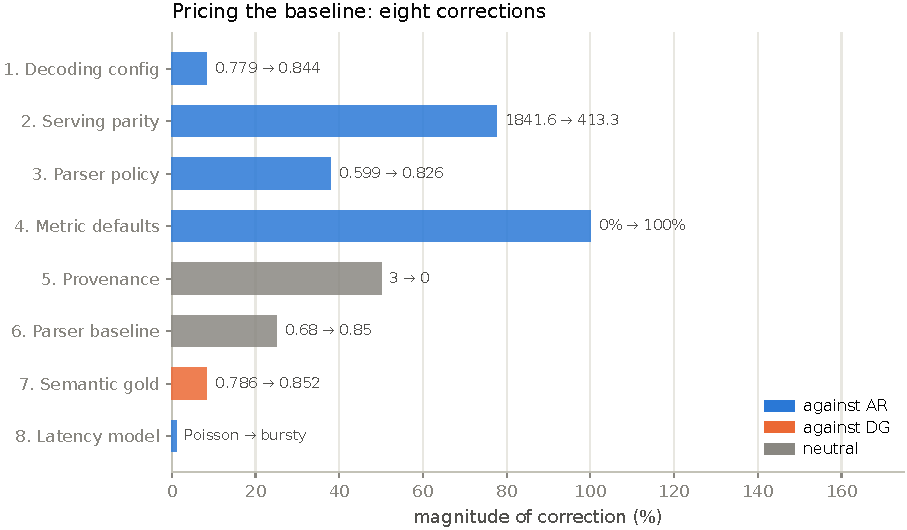
\includegraphics[width=\linewidth]{figures/fig8_defects.pdf}
\caption{Eight priced errors in our own comparison harness, each found by
re-reading committed artifacts
(\artifact{results/issue43\_nine\_field\_f1.json},
\artifact{results/issue44\_dg\_ksweep\_K*.json},
\artifact{results/issue66\_canvas\_*.json},
\artifact{results/issue68\_dg\_L*.json},
\artifact{results/issue49\_ar1b.json};
BGL, $n{=}300$ per cell). Five of eight biased against the
autoregressive arm. The clustering on one arm is the finding: a comparison
harness written by someone hoping the new architecture wins fails
asymmetrically.}
\label{fig:defects}
\end{figure}
